\chapter{Alimentation Forward}

La maquette d’étude comprend, outre le circuit de commande du transistor, le montage suivant :

\begin{figure}[h]
\centering
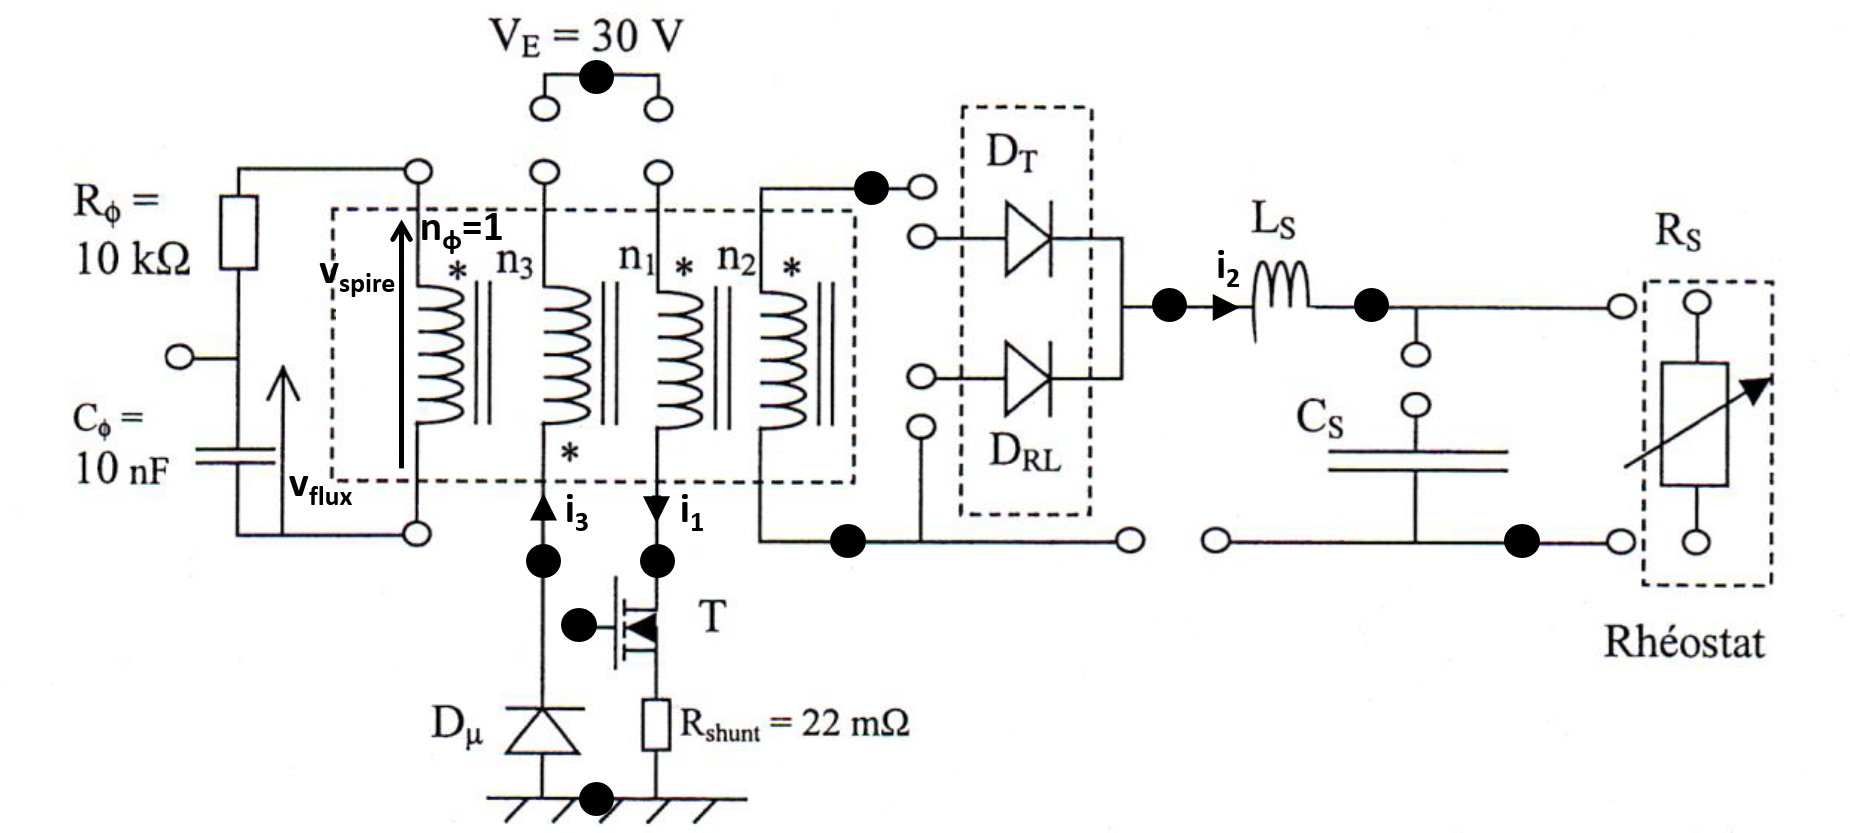
\includegraphics[width=\linewidth]{TP_Forward/fig/Schema_Forward.png}
%\caption{Simplified internal control}
\end{figure}

Des pointes de tests $\bullet$ permettent de visualiser les différents signaux, notamment le signal de commande du transistor MOSFET.

Les 4 enroulements sont sur le même noyau magnétique ETD29/16/10 réalisé avec une ferrite de type N27 dont la document est en annexe. Ce noyau peut être muni d’un entrefer réglé par des cales amagnétiques. Dans ce cas, la relation entre l’épaisseur $s$ de l’entrefer et la valeur $A_L$ de l’inductance spécifique est donnée par la relation suivante où $K_1$ et $K_2$ sont deux constantes données dans la documentation :
$$s=(\dfrac{A_L}{K_1})^{\dfrac{1}{K_2}}$$

Les liaisons manquantes devront être réalisées par des ``cavaliers'' permettant de visualiser les courants par l’utilisation de sondes appropriées. On veillera à \underline{\textbf{ne jamais déconnecter}} \underline{\textbf{l’enroulement de démagnétisation}}. Le rhéostat de charge peut être de 250 $\Omega$ ou 330 $\Omega$ indifféremment.



On notera la présence d’un circuit de mesure du flux réalisé par une spire unique reliée à un circuit R-C intégrateur. La tension $v_{flux}$ permet donc de visualiser l’ondulation du flux dans le circuit magnétique.

Le dispositif de commande du transistor est identique à celui de l’alimentation Flyback (Cf TP "Alimentation Flyback'')


\newpage
\section{Préparation}

On suppose que le transistor est commandé par un signal PWM de rapport cyclique $\alpha=0.25$. On suppose également que le convertisseur fonctionne en \textbf{régime de démagnétisation totale} pour le transformateur et qu'aucune charge n'est connectée en sortie du convertisseur. La tension d'entrée $V_E$ est supposée constante. On étudiera pour la préparation uniquement le \underline{régime permanent}.

\begin{enumerate}
\item Compléter les chronogrammes ci-dessous en traçant : 
\begin{itemize}
\item le flux $\varphi$ dans le transformateur
\item le courant $i_1$ délivré par l'alimentation
\item le courant $i_3$ dans l'enroulement de démagnétisation
\item la tension $v_2$ en sortie du transformateur
\end{itemize}


\begin{figure}[h]
\centering

\includegraphics[width=0.7\linewidth]{TP_Forward/fig/prepa.png}
%\caption{Simplified internal control}
\end{figure}

\item On suppose que la constante de temps du filtre $R_\phi-C_\phi$ est grande devant la période de découpage du hacheur. Montrer que $v_{flux}$ permet de visualiser l'ondulation de flux dans la transformateur. Déterminer l'ondulation de flux $\Delta \varphi$ en fonction de $\alpha$, $T$ et la valeur de $v_{spire}$ sur l'intervalle $0<t<\alpha T$.
\end{enumerate}


%%%%%%%%%%%%%%%%%

\newpage
Durant tout le TP, les précautions suivantes devront être prises :

\begin{itemize}
\item utiliser deux sources indépendantes pour réaliser $V_{alim}$ et l’alimentation ``de puissance'' $V_E$ : \textbf{on
règlera soigneusement la limitation de courant de celle-ci à 2 A}
\item laisser la tension $V_{alim}$ présente durant toute la séance mais baisser la tension $V_E$ à chaque
modification de branchement
\item ne pas abaisser la fréquence de découpage en dessous de 15 kHz
\item lorsque plusieurs mesures de tensions sont réalisées en même temps avec une sonde de tension, \textbf{attention à ne pas réaliser de court-circuit}. En effet, les sondes de tensions ne sont pas isolées entre elles, les références de potentiel des sondes sont donc liées via l'oscilloscope
\item \underline{\textbf{ne jamais déconnecter l’enroulement de démagnétisation}}
\end{itemize}

\section{Fonctionnement à vide}

Dans cette première partie de l’étude, il n’y a aucune charge en sortie de l’alimentation.

\begin{enumerate}
\item Régler la fréquence de découpage à 50 kHz et le rapport cyclique à sa valeur maximale (que l’on notera). Observer la tension aux bornes de la spire de mesure du flux $v_{spire}$ ainsi que la tension $v_{flux}$. En déduire l’excursion crête à crête $\Delta B$ de l'induction magnétique dans le circuit en s’aidant de la documentation ($\Delta B = B_{max} – B_{min}$).

\item Vérifier la démagnétisation complète à chaque période en observant simultanément les courants $i_1$ et $i_3$. Comparer ces observations à celle de la tension $v_{flux}$.

\item En observant simultanément le courant $i_1$ et la tension $v_1$, déterminer la valeur de l’inductance magnétisante au primaire, notée $L_1$. Quelle est la valeur de l’entrefer utilisé ?

\item Par comparaison des tensions vspire et $v_1$, puis $v_2$ et $v_3$ (les tensions $v_i$ sont mesurées aux bornes des bobinages de $n_i$ spires) déterminer les nombres de spires $n_1$, $n_2$ et $n_3$. Ce résultat est-il cohérent avec la valeur de $L_1$ trouvée (utiliser la documentation du noyau magnétique) ?

\item En observant simultanément le courant $i_1$ et la tension $v_{flux}$, diminuer progressivement la fréquence de découpage jusqu’à 20 kHz tout en maintenant le rapport cyclique maximal. Que se passe-t-il ?
\end{enumerate}

\newpage
\section{Fonctionnement en charge}

On connecte le rhéostat de charge après l’avoir régler à une valeur de $30\Omega$  pour effectuer les mesures suivantes. Il ne faut pas oublier de connecter toutes les liaisons ``ouvertes'' permettant les mesures des différents courants au secondaire. On règle de nouveau la fréquence de découpage à 50 kHz et le rapport cyclique à sa valeur maximale.

\begin{enumerate}
\item Observer simultanément puis successivement les couples de grandeurs suivants :
\begin{itemize}
\item la tension secondaire $v_2$ et la tension aux bornes de $D_{RL}$, $v_{DRL}$
\item le courant de sortie $i_S$ et la tension aux bornes de $D_{RL}$
\item les courants dans les deux diodes secondaires, $i_{DRL}$ et $i_{DT}$
\end{itemize}

Que peut-on dire du mode de fonctionnement de ces diodes secondaires ?

\item Observer simultanément le courant $i_{LS}$ dans la bobine $L_S$ et la tension $v_{DRL}$. En déduire la valeur de cette inductance de sortie $L_S$. Que peut-on dire de son dimensionnement ?

\item Observer simultanément le courant dans le condensateur de filtrage $i_{CS}$ et la tension de sortie $v_S$. En déduire la valeur du condensateur de filtrage $C_S$.

\end{enumerate}

\section{Courbes statiques}

Le but de ces mesures est de relever le réseau des caractéristiques statiques en sortie de l’alimentation. La fréquence de découpage est maintenue constante égale à 50 kHz.

\begin{enumerate}
\item Pour plusieurs valeurs du rapport cyclique (par exemple $\alpha_{max}$, 0.3, 0.2, 0.1), modifier la résistance du rhéostat de charge pour faire varier le courant moyen débité entre sa valeur minimale (obtenue avec le rhéostat au maximum) et une valeur maximale de 2 A. Relever alors les valeurs moyennes du courant débité par l’alimentation de puissance $V_E$, $I_E$, du courant de sortie, $I_S$, et de la tension de sortie, $V_S$.


\item En déduire le tracé des caractéristiques $V_S(I_S)$ paramétrées par $\alpha$. Tracer également les caractéristiques de transfert en puissance $P_S(P_E)$ et en déduire le rendement.
\end{enumerate}
